\section{Low-Pass filter}

%Inde i lys-sensoren sidder der en transistor i en spændingsdeling. Denne transistor kan generere noget høj frekvent støj. Dette filtrers væk med et low-pass filter. 
Et low-pass filter er et filter som sorterer høje frekvenser fra men samtidig tillader DC (jævnstrøm) igennem.

\begin{figure}[h!]
  \centering
  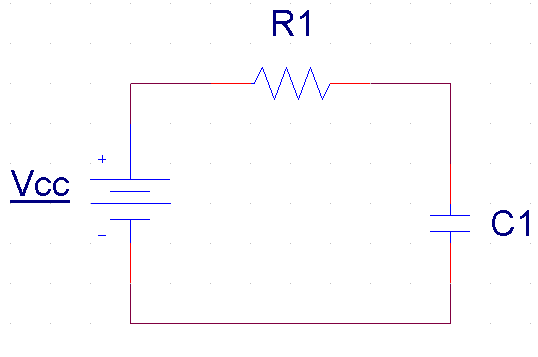
\includegraphics[width=0.6\textwidth]{figures/low_pass_schematic.png}
\end{figure}

Et low-pass filter kan konstrueres med en modstand og en kondensator i serie. Kondensatoren er forbundet til stel så den skaber en AC-kortslutning (vekselsstrøm) og derved filtrer AC væk fra signalet. 
Lave frekvenser filtreres ikke væk, fordi kondensatoren bruger tid til at lade op og derved ikke længere fungerer som stel fra de frekvenser.

\begin{figure}[h!]
  \centering
  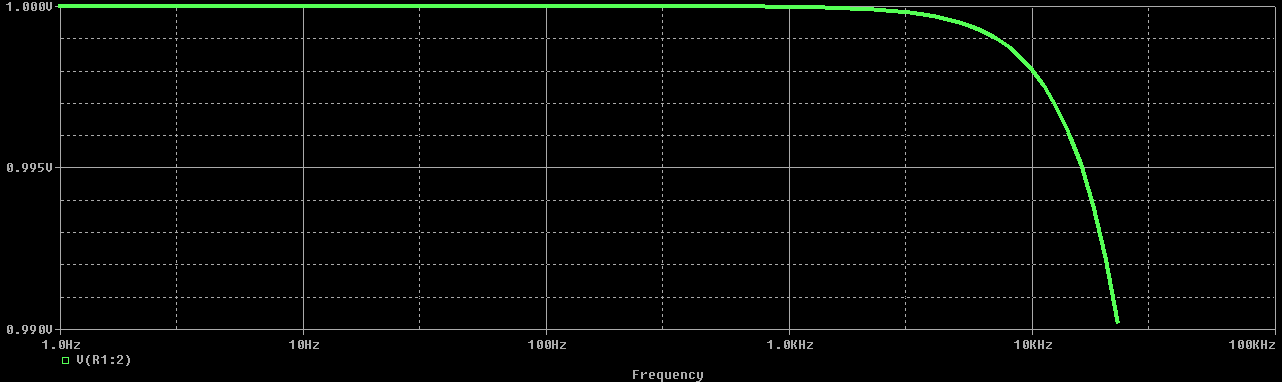
\includegraphics[width=0.6\textwidth]{figures/low_pass_cut_off_frequency.png}
  \caption{Eksempel på low-pass filter med 1k modstand og 1nF kondensator.}
\end{figure}
Som det ses på low-pass filteret ovenover\fxnote{find ud af hvordan vi skal referer til figur} hvor frekvenser omkring 1k begynder at blive skåret fra.
